\documentclass{article}
\usepackage[utf8]{inputenc}
\textheight = 25cm 
\textwidth = 15cm
\topmargin = -2.5cm 
\oddsidemargin = 1.5cm
\usepackage{float}
\usepackage{graphicx}
\graphicspath{{./images/}}

\usepackage{amsmath}
\usepackage{mathtools, xparse}
\usepackage[shortlabels]{enumitem}
\usepackage[most]{tcolorbox}
\usepackage{adjustbox}
\usepackage{bm} 

\DeclarePairedDelimiter{\norm}{\lVert}{\rVert}

\title{Tarea 6 Mecánica Analítica}
\author{Cerritos Lira Carlos}
\date{28 de Marzo del 2020}

\begin{document}
\maketitle
\section*{Problemas}
\section*{1.-}
\subsubsection*{3.4)}
Un niño monta un "caballito" que sube y baja sinusoidalemtne $h=h_0sin(wt)$ con 
relación a un tiovivo que gira alrededor de la vertical con una velocidad(tangencial)
constante $\Omega$. si el niño está a una distancia $c$ del eje de rotación, 
hallése una expresión de su aceleración relativa al suelo en funcion de $\Omega, c, h_0, w$ 
y $t$. 
\begin{tcolorbox}[breakable]
    Definimos dos sistemas, $S$ en resposo en el centro del juego y $S'$ justo debajo del 
    caballito como en la figura:
    \begin{figure}[H]
        \centering
        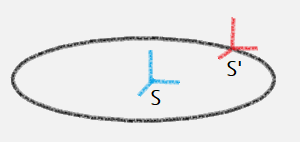
\includegraphics[]{p1_horse.png}
    \end{figure}
    definimos los vectores:
    \begin{align*}
        \bm{e_r} &= cos(\Omega t) \bm{i} + sin(\Omega t) \bm{j} \\ 
        \bm{e_\theta} &= sin(\Omega t)\bm{i} - cos(\Omega t) \bm{j}
    \end{align*}
    Sea $\bm{r}$ la función de posición en el sistema $S$, se tiene:
    \begin{align*}
        \bm{r} 
        &= \bm{R'} + \bm{r'} \\
        &= c\bm{e_r} + h_0sin(wt)\bm{k} \\
        \bm{v} &= -c\Omega\bm{e_\theta} + h_0wcos(wt)\bm{k} \\
        \bm{a} &= -c\Omega^2\bm{e_r} - h_0w^2sin(wt)\bm{k} \\
    \end{align*}
\end{tcolorbox}

\section*{2.-}
\subsubsection*{4.2)}
Encontrar la posición en un tiempo $t$ de una partícula de masa $m$, cuando la fuerza aplicada
es $F=2mcos(wt)$ y $x=8$ a $t=0$ y $x=-b$ a $t=\frac{\pi}{2w}$.
\begin{tcolorbox}[breakable]
    Tenemos la siguiente información:
    \begin{align*}
        a &= 2cos(wt)  \\
        v &= \frac{2}{w}sin(wt) + v(0)  \\ 
        x &= -\frac{2}{w^2}cos(wt) + v(0)t + \frac{2}{w^2} + x(0) 
    \end{align*}
    donde 
    \[x(0) = 8 \]
    podemos encontrar el valor de $v(0)$ mediante la relación $x(\frac{\pi}{2w}) = -b$
    , de donde obtenemos:
    \begin{align*}
        v(0) &= -\frac{\frac{2}{w^2} + 8 + b}{\frac{\pi}{2w}}
    \end{align*}
\end{tcolorbox}

\section*{3.-}
\subsubsection*{4.4)}
\begin{enumerate}[a)]
    \item Si la velocidad límite de caída de un hombre de $80kg$, con paracaídas, es 
    la misma que tendría al caer libremente $0.75m$; hallar el valor de esta velocidad 
    límite y la constante de amortiguamiento $k$ (supóngase $F_{amort} = -mkv$)
    \item Supongamos ahora que el hombre cae libremente (partiendo del reposo) durante 
    5 segundos y que después abre su paracaídas. Luego de otros 5 segundos, ¿cual será su 
    velocidad? 
\end{enumerate}
\begin{tcolorbox}[breakable]
    \subsubsection*{Caida con paracaídas}
    Sea $v$ la función de velocidad del hombre en caída libre con paracaídas, donde se elige 
    un sistema de referencia tal que $x(0)=0, v(t_0) = v_0$, de acuerdo al problema se 
    satisface la ecuación diferencial:
    \begin{align*}
        v' &= g - kv 
    \end{align*}
    que tiene por solución:
    \begin{align*}
        v &= \frac{g}{k} + \left(v_0 - \frac{g}{k}\right)e^{-kt}
    \end{align*}
    vemos que cuando $t \to \infty$ se cumple:
    \begin{align*}
        v_t = \frac{g}{k}
    \end{align*}
    \subsubsection*{a)}
    La velocidad y posición en caída libre son:
    \begin{align*}
        v &= gt \\
        x &= \frac{g}{2}t^2 
    \end{align*}
    el tiempo que transcurre cuando se recorre una distancia $x_0$ es:
    \begin{align*}
        t_0 
        &= \sqrt{\frac{2}{g}x_0} 
    \end{align*}
    la velocidad que se alcanza es:
    \begin{align*}
        v_t 
        &= \sqrt{2gx_t} = 3.836 \left[ \frac{m}{s^2} \right]
    \end{align*}
    despejando $k$ obtenemos:
    \begin{align*}
        k 
        &= \frac{g}{v_t} = 2.557 [s^{-1}]
    \end{align*}
    \subsubsection*{b)}
    La velocidad para $t>5$ esta dada por:
    \begin{align*}
        v 
        &= \frac{g}{k} + \left( 5g - \frac{g}{k} \right)e^{-k(t-5)}  \\ 
        v(10)
        &= 3.847 \left[ \frac{m}{s^2} \right]
    \end{align*}
\end{tcolorbox}

\section*{4.-}
\subsubsection*{4.7)}
Una partícula de masa $m$ tiene aplicada una fuerza $F=-kx^2$. Si $\dot{x} = v_0$ 
cuando $x=0$, hállese:
\begin{enumerate}[a)]
    \item la ecuación de la energía
    \item el punto de retorno
    \item la velocidad en cualquier posición
\end{enumerate} 
\begin{tcolorbox}[breakable]
    \subsubsection*{a)}
    Encontramos una energía potencial que satisface $U(0) = 0$ usando la relación:
    \begin{align*}
        U(x)
        &= -\int_0^x F(x')dx' \\
        &= \frac{k}{3}x^3  
    \end{align*}
    por el teorema del trabajo y la energía se tiene la relación:
    \begin{align*}
        U + K &= U(0) + K(0) \\
        \frac{k}{3}x^3 + \frac{1}{2}m\dot{x}^2 &= \frac{1}{2}mv_0^2 = E
    \end{align*}
    \subsubsection*{b)}
    En el punto de retorno se satisface $U = E \implies \dot{x} = 0$, 
    despejando $x$ de la ecuación de energía obtenemos:
    \begin{align*}
        x &= \left(\frac{3m}{2k}v_0^2\right)^{\frac{1}{3}}
    \end{align*} 
    \subsubsection*{c)}
    Despejando $\dot{x}$ de la ecuación de energía obtenemos:
    \begin{align*}
        \dot{x} &= \sqrt{v_0^2 - \frac{2k}{3m}x^3}
    \end{align*} 
\end{tcolorbox}

\section*{5.-}
\subsubsection*{3.3)}
Un semicilindro se balance sinusoidalmente sin deslizamiento, como se muestra en la figura 
$3-11$, de tal forma que $\theta = sin2t$. 
\begin{enumerate}[a)]
    \item Cuando pasa por la posición neutra $\theta=0$, ¿cuál es la aceleración del punto
    de contacto con la superfice fija?
    \item Cuando el semicilindro está al ángulo máximo de 1 radían ¿cuál es la aceleración 
    del punto de contacto con la superficie fija?
\end{enumerate}

\begin{tcolorbox}[breakable]
    \subsubsection*{Caso general}
    Definimos dos sistemas como en la imagen:
    \begin{figure}[H]
        \centering 
        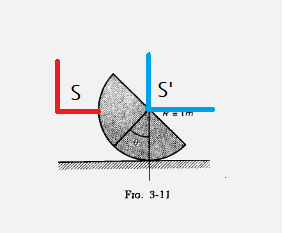
\includegraphics[trim=20 20 20 20, clip]{p5_cylinder.png}
    \end{figure}
    Sea $\bm{r}$ la función de posición en el sistema $S$ para el punto que se hace de contacto al tiempo $t_0$,
    como se balancea sin deslizamiento:
    \begin{align*}
        \bm{R} &= \theta \bm{i} \\
        \bm{r'} &= sin(\theta_0-\theta)\bm{i} - cos(\theta_0-\theta)\bm{j}
    \end{align*}
    El movimiento respecto al sistema en reposo $S$, está dado por:
    \begin{align*}
        \bm{r} &= \bm{R} + \bm{r'} \\
        \bm{v} &=\dot{\theta}\bm{i} 
        - \dot{\theta}cos(\theta_0-\theta)\bm{i} 
        - \dot{\theta}sin(\theta_0-\theta)\bm{j} \\ 
        \bm{a} 
        &=\ddot{\theta}\bm{i} 
        -(\ddot{\theta}cos(\theta_0-\theta) + \dot{\theta}^2sin(\theta_0-\theta))\bm{i} 
        -(\ddot{\theta}sin(\theta-\theta_0) - \dot{\theta}^2cos(\theta_0-\theta))\bm{j}  
    \end{align*}
    La aceleración de este punto cuando se hace de contacto es:
    \begin{align*}
        \bm{a}(t_0) 
        &= \ddot{\theta}(t_0)\bm{i} - \ddot{\theta}(t_0)\bm{i} + \dot{\theta^2}(t_0)\bm{j} \\
        &= 4cos^2(2t_0)\bm{j} \left[ \frac{m}{s^2} \right]
    \end{align*}
    \subsubsection*{a)}
    En este caso $t_0 = 0[s]$, sustituyendo obtenemos:
    \begin{align*}
        \bm{a} &= 4\bm{j} \left[ \frac{m}{s^2} \right]
    \end{align*}
    \subsubsection*{b)}
    En este caso tenemos $t_0 = \frac{\pi}{4}[s]$, sustituyendo obtenemos:
    \begin{align*}
        \bm{a} &= \bm{0} \left[ \frac{m}{s^2} \right]
    \end{align*}
\end{tcolorbox}
\end{document}
